\documentclass[tikz,border=8pt]{standalone}
% Shared look for every TikZ diagram. Load with \input{../../tools/tikz-style.tex}
\usepackage[T1]{fontenc}
\usepackage{lmodern}
\renewcommand{\sfdefault}{lmr}  % diagrams use the same serif as the text
\usetikzlibrary{arrows.meta, positioning, shapes.geometric, calc, fit, backgrounds}
\definecolor{cblue}{HTML}{4C78A8}
\definecolor{corange}{HTML}{F58518}
\definecolor{cgreen}{HTML}{54A24B}
\definecolor{cred}{HTML}{E45756}
\definecolor{cpurple}{HTML}{B279A2}
\definecolor{cgrey}{HTML}{6B6B6B}
\tikzset{
  every picture/.style={font=\sffamily, line width=1.2pt},
  box/.style={draw=#1, fill=#1!12, rounded corners=4pt, align=center, inner sep=7pt, minimum height=1.1cm},
  box/.default=cgrey,
  arrow/.style={-{Stealth[length=3mm]}, draw=cgrey, line width=1.4pt},
  title/.style={font=\sffamily\bfseries\Large},
  note/.style={font=\sffamily\small, text=cgrey, align=center},
}
\AtBeginDocument{\hyphenpenalty=10000 \exhyphenpenalty=10000}

\begin{document}
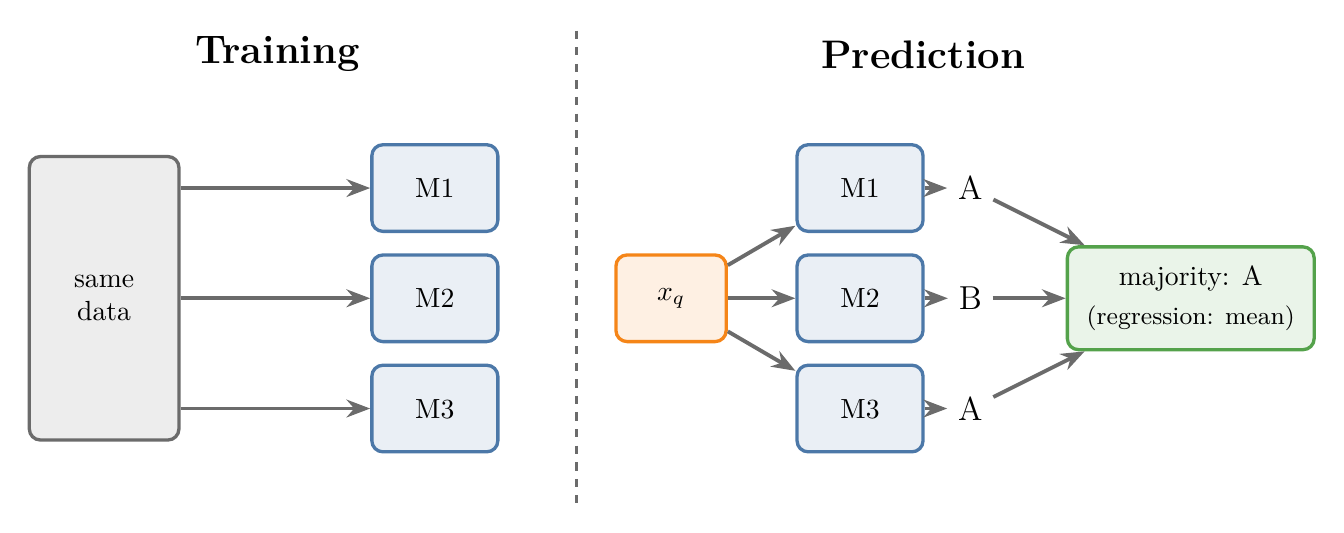
\begin{tikzpicture}[m/.style={box=cblue, minimum width=1.6cm}]
  \node[title] at (2.2,3.1) {Training};
  \node[box=cgrey, minimum height=3.6cm, minimum width=1.9cm] (d) at (0,0) {same\\data};
  \foreach \i/\y in {1/1.4, 2/0, 3/-1.4} {
    \node[m] (t\i) at (4.2,\y) {M\i};
    \draw[arrow] (d.east |- t\i) -- (t\i);
  }
  \draw[cgrey, dashed] (6.0,3.4) -- (6.0,-2.6);
  \node[title] at (10.4,3.1) {Prediction};
  \node[box=corange, minimum width=1.4cm] (q) at (7.2,0) {$x_q$};
  \foreach \i/\y/\v in {1/1.4/A, 2/0/B, 3/-1.4/A} {
    \node[m] (p\i) at (9.6,\y) {M\i};
    \draw[arrow] (q) -- (p\i);
    \node[font=\sffamily\large] (v\i) at (11.0,\y) {\v};
    \draw[arrow] (p\i) -- (v\i);
  }
  \node[box=cgreen, align=center] (out) at (13.8,0) {majority: A\\[2pt]\small (regression: mean)};
  \foreach \i in {1,2,3} \draw[arrow] (v\i) -- (out);
\end{tikzpicture}
\end{document}
